\providecommand{\setflag}{\newif \ifwhole \wholefalse}
\setflag
\ifwhole\else

% Typography and geometry ----------------------------------------------------
\documentclass[letterpaper]{scrbook}
\usepackage[inner=3cm,top=2.5cm,outer=3.5cm]{geometry}

\renewcommand\familydefault{bch}
\usepackage[utf8]{inputenc}
\usepackage{microtype}
\usepackage[small]{caption}
\usepackage[small]{titlesec}
\raggedbottom

% Graphics -------------------------------------------------------------------
\usepackage[pdftex]{graphicx}
\graphicspath{{_include/}}
\DeclareGraphicsExtensions{.png,.pdf}

% Code formatting ------------------------------------------------------------
\usepackage{fancyvrb}
\usepackage{courier}
\usepackage{listings}
\usepackage{color}
\usepackage{alltt}


\definecolor{comment}{rgb}{0.60, 0.60, 0.53}
\definecolor{background}{rgb}{0.97, 0.97, 1.00}
\definecolor{string}{rgb}{0.863, 0.066, 0.266}
\definecolor{number}{rgb}{0.0, 0.6, 0.6}
\definecolor{variable}{rgb}{0.00, 0.52, 0.70}
\lstset{
  basicstyle=\ttfamily,
  keywordstyle=\bfseries, 
  identifierstyle=,  
  commentstyle=\color{comment} \emph,
  stringstyle=\color{string},
  showstringspaces=false,
  columns = fullflexible,
  backgroundcolor=\color{background},
  mathescape = true,
  escapeinside=&&,
  fancyvrb
}
\newcommand{\code}[1]{\lstinline!#1!}
\newcommand{\f}[1]{\lstinline!#1()!}



% Links ----------------------------------------------------------------------

\usepackage{hyperref}
\definecolor{slateblue}{rgb}{0.07,0.07,0.488}
\hypersetup{colorlinks=true,linkcolor=slateblue,anchorcolor=slateblue,citecolor=slateblue,filecolor=slateblue,urlcolor=slateblue,bookmarksnumbered=true,pdfview=FitB}
\usepackage{url}

% Tables ---------------------------------------------------------------------
\usepackage{longtable}
\usepackage{booktabs}

% Miscellaneous --------------------------------------------------------------
\usepackage{pdfsync}
\usepackage{appendix}

\usepackage[round,sort&compress,sectionbib]{natbib}
\bibliographystyle{plainnat}


\title{ggplot2}
\author{Hadley Wickham}

\begin{document}
\fi


% SET_DEFAULTS
%   GG-WIDTH: 4  GG-HEIGHT: 4
%   TEX-WIDTH: 0.5\textwidth
%   INLINE: FALSE
%   CACHE: TRUE
% 

% END

\chapter{Mastering the grammar}
\label{cha:mastery}

\section{Introduction}

You can choose to use just \f{qplot}, without any understanding of the underlying grammar, but you will not be able to use the full power of ggplot.  By learning more about the grammar, and the components that make it up, you will be able to create a wider range of plots, as well as being able to combine multiple sources of data, and customise to your heart's content.  You may want to skip this chapter in a first reading of the book, coming back to it when you want a deeper understanding of how all the pieces fit together.

This chapter describes the theoretical basis of \ggplot: the layered grammar of graphics.  The layered grammar is based on Wilkinson's grammar of graphics \citep{wilkinson:2006}, but adds a number of enhancements that help it to be more expressive and fit smoothly into the R environment.  The differences between the layered grammar and Wilkinson's grammar are described fully in \citep{wickham:2008}, and a guide for converting between {\sc gpl} and \ggplot is included in Appendix~\ref{chp:translating}.  In this chapter you will learn a little bit about each component of the grammar and how they all fit together.  The next chapters discuss the components in more detail, and provide more examples of how you can use them in practice.

This chapter begins by describing in detail the process of drawing a simple plot.  Section~\ref{sec:simple-plot} start with a simple scatterplot, then in Section~\ref{sec:complex-plot} make it more complex by adding a smooth line and faceting.  While working through these examples you will be introduced to all six components of the grammar, which are then defined more precisely in Section~\ref{sec:components}.  The chapter concludes with Section~\ref{sec:data-structures}, which describes how the various components map to data structures in R.  

\section{Fuel economy data}
\label{sec:fuel_economy_data}

Consider the fuel economy dataset illustrated in Table~\ref{tbl:mpg}.  It records make, model, class, engine size, transmission and fuel economy for a selection of US cars in 1999 and 2008.  It contains the 38 models that had a new release every year, an indicator that the car was a popular model.  These models are the Audi A4, Audi A4 Quattro, Audi A6 Quattro, Chevrolet C1500 Suburban 2wd, Chevrolet Corvette, Chevrolet K1500 Tahoe 4wd, Chevrolet Malibu, Dodge Caravan 2wd, Dodge Dakota Pickup 4wd, Dodge Durango 4wd, Dodge Ram 1500 Pickup 4wd, Ford Expedition 2wd, Ford Explorer 4wd, Ford F150 Pickup 4wd, Ford Mustang, Honda Civic, Hyundai Sonata, Hyundai Tiburon, Jeep Grand Cherokee 4wd, Land Rover Range Rover, Lincoln Navigator 2wd, Mercury Mountaineer 4wd, Nissan Altima, Nissan Maxima, Nissan Pathfinder 4wd, Pontiac Grand Prix, Subaru Forester Awd, Subaru Impreza Awd, Toyota 4runner 4wd, Toyota Camry, Toyota Camry Solara, Toyota Corolla, Toyota Land Cruiser Wagon 4wd, Toyota Toyota Tacoma 4wd, Volkswagen Gti, Volkswagen Jetta, Volkswagen New Beetle, and Volkswagen Passat.  This data was collected from the EPA fuel economy website, \url{http://fueleconomy.gov}.

% source("latex.r")
% cat(tabulate(mpg[1:10, -6]))
\begin{table}
  \begin{center}
  \begin{tabular}{llrrrlrrl}
    \toprule
    manufacturer & model & disp & year & cyl & cty & hwy & class \\
    % Model & Manufacturer & Displacement (l) & Year & Cylinders & City mpg & Highway mpg & Class \\
    \midrule
    audi & a4         & 1.8 & 1999 & 4 & 18 & 29 & compact\\
    audi & a4         & 1.8 & 1999 & 4 & 21 & 29 & compact\\
    audi & a4         & 2.0 & 2008 & 4 & 20 & 31 & compact\\
    audi & a4         & 2.0 & 2008 & 4 & 21 & 30 & compact\\
    audi & a4         & 2.8 & 1999 & 6 & 16 & 26 & compact\\
    audi & a4         & 2.8 & 1999 & 6 & 18 & 26 & compact\\
    audi & a4         & 3.1 & 2008 & 6 & 18 & 27 & compact\\
    audi & a4 quattro & 1.8 & 1999 & 4 & 18 & 26 & compact\\
    audi & a4 quattro & 1.8 & 1999 & 4 & 16 & 25 & compact\\
    audi & a4 quattro & 2.0 & 2008 & 4 & 20 & 28 & compact\\
        \bottomrule
  \end{tabular}
  \end{center}
  \caption{The first 10 cars in the \code{mpg} data set, included in the \ggplot package.  \var{cty} and \var{hwy} record miles per gallon (mpg) for city and highway driving respectively.  }
  \label{tbl:mpg}
\end{table}

This dataset suggests many interesting questions.  How are engine size and fuel economy related?  Has fuel economy improved in the last ten years?  We will try to answer the first question and in the process learn more detail about how the scatterplot is created.

\section{Building a scatterplot}
\label{sec:simple-plot}

Consider Figure~\ref{fig:mpg}, one attempt to answer this question.  It is a scatterplot of two continuous variables (engine displacement and highway mpg), with points coloured by a third variable (number of cylinders).  From your experience in the previous chapter, you should have a pretty good feel for how to create this plot with \f{qplot}.  But what is going on underneath the surface?  How does \ggplot draw this plot?

% FIGURE
%   LABEL: mpg
%   GG-WIDTH: 8 GG-HEIGHT: 4 TEX-WIDTH: \textwidth
%   CAPTION: A scatterplot of engine displacement in litres (displ) vs
%   average highway miles per gallon (hwy).  Points are coloured according
%   to number of cylinders.  This plot summarises the most important
%   factor governing fuel economy: engine size
% 
% qplot(displ, hwy, data=mpg, colour=factor(cyl))
% 
\input{_include/b456d52cc6c3828652aafc872cb47070.tex}
% END

\subsubsection{Mapping aesthetics to data}

What is a scatterplot?  You have seen many before and have probably even drawn some by hand.  A scatterplot represents each observation as a point (•), positioned according the value of two variables.  As well as a horizontal and vertical position, each point also has a size, a colour and a shape. In a basic scatterplot these properties are usually constant (i.e.\ each point has the same size, colour and shape), but they can also be mapped to a variable.  These attributes are called called {\bf aesthetics}, and are the properties that can perceived on the graphic.  Each aesthetic can be mapped to a variable, or set to a constant value.  In Figure~\ref{fig:mpg} $x$-position is mapped to \var{displ}, $y$-position to \var{hwy} and colour to \var{cyl}.  Size and shape are not mapped to variables, but remain at their (constant) default values.  

Once we have these mappings we can create a new dataset that records this information.  Table~\ref{tbl:mapping} shows the first 10 rows of the data behind Figure~\ref{fig:mpg}.  This new dataset encapsulates the combination of the original data and the aesthetic mappings.  We can create many different types of plots using this data.  The scatterplot uses points, but we were instead to draw lines we would get a line plot.  If we used bars, we'd get a bar plot.  Neither of those examples make sense for this data, but we could still draw them, as in Figure~\ref{fig:other-geoms}.  Much like in English, we can produce many grammatically valid plots that don't make any sense.

% scatter <- with(mpg, data.frame(x = displ, y = hwy, colour = cyl))
% cat(tabulate(scatter[1:10, ]))
\begin{table}[ht]
  \begin{center}
  \begin{tabular}{rrr}
    \toprule
    \code{x} & \code{y} & \code{colour}\\
    \midrule
    1.8 & 29 & 4\\
    1.8 & 29 & 4\\
    2.0 & 31 & 4\\
    2.0 & 30 & 4\\
    2.8 & 26 & 6\\
    2.8 & 26 & 6\\
    3.1 & 27 & 6\\
    1.8 & 26 & 4\\
    1.8 & 25 & 4\\
    2.0 & 28 & 4\\
    \bottomrule
  \end{tabular}
  \end{center}
  \caption{First 10 rows from \code{mpg} rearranged into format for scatterplot.  This is all the information we need to draw the scatterplot.}
  \label{tbl:mapping}
\end{table}

% FIGURE
%   LABEL: other-geoms
%   CAPTION: Instead of using points to represent the data, we could use
%   other geoms like, \leftc lines or, \rightc bars.  Neither of these geoms
%   make much sense for this data, but they are still valid graphics.
% 
% qplot(displ, hwy, data=mpg, colour=factor(cyl), geom="line") + 
%   opts(drop = "legend_box")
% qplot(displ, hwy, data=mpg, colour=factor(cyl), geom="bar", 
%   stat="identity", position = "identity") + 
%   opts(drop = "legend_box")
\input{_include/f3d7e4c704d09556e29315c4a638c996.tex}
% END

Bars, lines and points are all examples of geometric objects, or {\bf geom}s. Geoms determine the ``type'' of the plot. Plots that use a single geom are often given a special name, a few of which are listed in Table~\ref{tbl:named-plots}. More complex plots with combinations of multiple geoms don't have a special name, and we have to describe them by hand. For example, Figure~\ref{fig:complex-plot} overlays a per group regression line on the existing plot. What would you call this plot?   Once you've mastered the grammar, I think you'll find that most of the plots that you produce are uniquely tailored to your problems and will no longer have common names.

\begin{table}
  \begin{center}
  \begin{tabular}{lll}
    \toprule 
    Named plot & Geom & Other features \\
    \midrule
    scatterplot & point &  \\
    bubblechart & point & size mapped to a variable \\ 
    barchart & bar &  \\
    box and whiskers plot & boxplot &  \\
    line chart & line &  \\     
    \bottomrule
  \end{tabular}
  \end{center}
  \caption{A selection of named plots and the geoms that they correspond to.}
  \label{tbl:named-plots}
\end{table}

% FIGURE
%   LABEL: complex-plot
%   GG-WIDTH: 8 GG-HEIGHT: 4 TEX-WIDTH: \textwidth
%   CAPTION: More complicated plots don't have their own names.  This plot
%   takes Figure~\ref{fig:mpg} and adds a regression line to each group. 
%   What would you call this plot?
% 
% qplot(displ, hwy, data=mpg, colour=factor(cyl)) + 
% geom_smooth(data= subset(mpg, cyl != 5), method="lm")
\input{_include/1e64e4f26f78be4188c72c485f3a5dad.tex}
% END

\subsubsection{Scaling} 

The values in Table~\ref{tbl:mapping} have no meaning to the computer.  We need to convert them from data units (e.g.\ litres, miles per gallon and number of cylinders) to physical units (e.g.\ pixels and colours) that the computer can display.  This conversion process is called {\bf scaling} and performed by (surprise!) scales.   Appendix~\ref{chp:specification} describes the way that specifies values for colours, sizes, shapes and so on.

For scales that control the horizontal and vertical position, we need an additional step which determines how the two positions (x and y) combine to form the final position on the plot.  This is done by the coordinate system, or {\bf coord}.  In most cases this will be Cartesian coordinates, but it might by polar coordinates, or a spherical projection used for a map.

Scaling position is easy in this example because we are using the default  linear scales and Cartesian coordinate system.  We only need a linear mapping from the range of the data to $[0, 1]$.  We use $[0, 1]$ instead of exact pixels because the drawing system that \ggplot uses, \code{grid}, takes care of that final conversion. 

The process for mapping the colour is a little more complicated, as we have a  non-numeric result: colours.  However, colours can be parameterised numerically, typically with three values.  For discrete values, the default colour scale maps the  to evenly spaced hues on a colour wheel, as shown in  Figure~\ref{fig:colour-wheel}.

\begin{figure}[htbp]
  \centering
    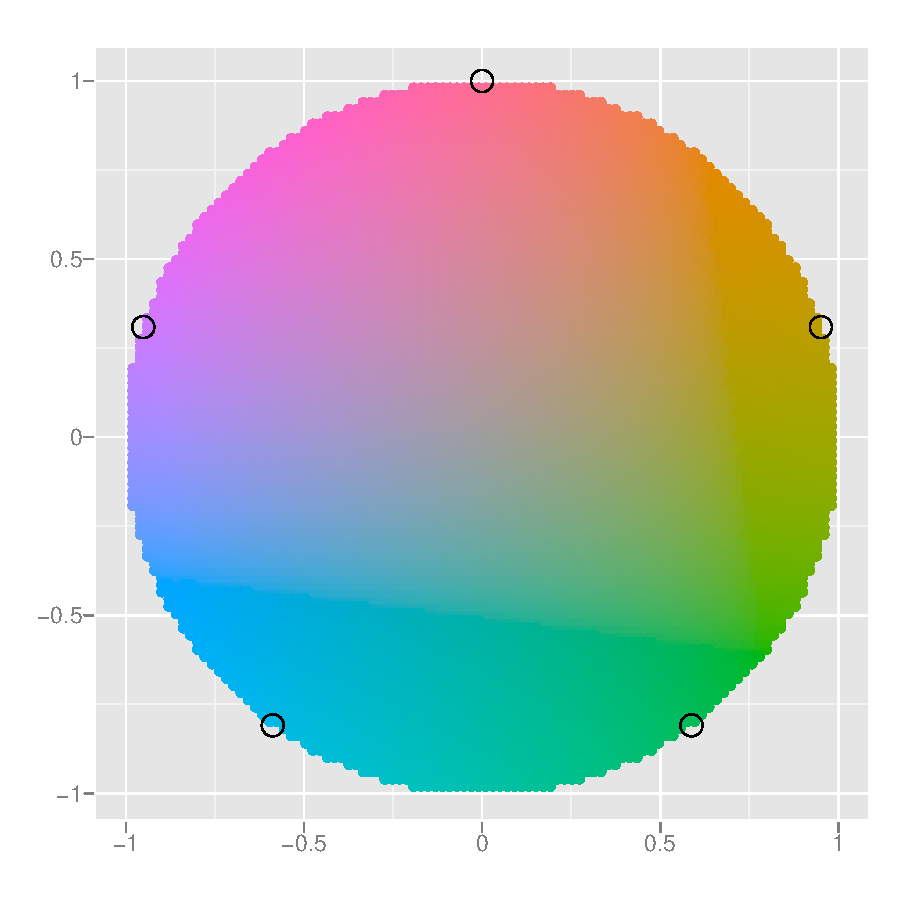
\includegraphics[width=3in]{colour-wheel.pdf}
  \caption{A colour wheel showing how the default colour scheme for discrete values is produced.}
  \label{fig:colour-wheel}
\end{figure}

The result of these conversions is Table~\ref{tbl:scaled}, which contains values that have meaning to the computer.  As well as the variables from the aesthetic mapping, we have also included the default values for the geom.  We need these so that the aesthetics for each point are completely specified.

% Colour the entries by their actual colour

% scaled <- transform(scatter,
%   x = format(rescaler(x, "range"), digits=2),
%   y = format(rescaler(y, "range"), digits=2)
% )
% col <- scale_colour_discrete()
% col$train(factor(scaled$colour))
% scaled$colour <- col$map(factor(scaled$colour))
% scaled$size <- 1
% scaled$shape <- 20
% cat(tabulate(scaled[1:10, ]))

\definecolor{ff6c91}{rgb}{1.00, 0.42, 0.57}
\definecolor{00c1a9}{rgb}{0.00, 0.76, 0.66}

\begin{table}[ht]
  \begin{center}
  \begin{tabular}{rrrrr}
    \toprule
    \code{x} & \code{y} & \code{colour} & \code{size} & \code{shape}\\
    \midrule
    0.037 & 0.531 & {\color{ff6c91} \#FF6C91} & 1 & 20 \\
    0.037 & 0.531 & {\color{ff6c91} \#FF6C91} & 1 & 20 \\
    0.074 & 0.594 & {\color{ff6c91} \#FF6C91} & 1 & 20 \\
    0.074 & 0.562 & {\color{ff6c91} \#FF6C91} & 1 & 20 \\
    0.222 & 0.438 & {\color{00c1a9} \#00C1A9} & 1 & 20 \\
    0.222 & 0.438 & {\color{00c1a9} \#00C1A9} & 1 & 20 \\
    0.278 & 0.469 & {\color{00c1a9} \#00C1A9} & 1 & 20 \\
    0.037 & 0.438 & {\color{ff6c91} \#FF6C91} & 1 & 20 \\
    0.037 & 0.406 & {\color{ff6c91} \#FF6C91} & 1 & 20 \\
    0.074 & 0.500 & {\color{ff6c91} \#FF6C91} & 1 & 20 \\
    \bottomrule
  \end{tabular}
  \end{center}
  \caption{Simple dataset with variables mapped into aesthetic space.  Default values for other aesthetics are also included: the points will be filled circles (shape 20 in R) with a 1mm diameter.}
  \label{tbl:scaled}
\end{table}

Finally, we need to render this data to create the graphical objects that are displayed on the screen.  To create a complete plot we need to combine graphical objects from three sources:  \emph{data}, represented by the point geom; \emph{scales and coordinate system}, which generate axes and legends so that we can read values from the graph; and \emph{plot annotations}, such as the background and plot title.  Figure~\ref{fig:empty} removes the contribution of the data to show what elements the scales and plot contribute.

\begin{figure}[htbp]
  \centering
  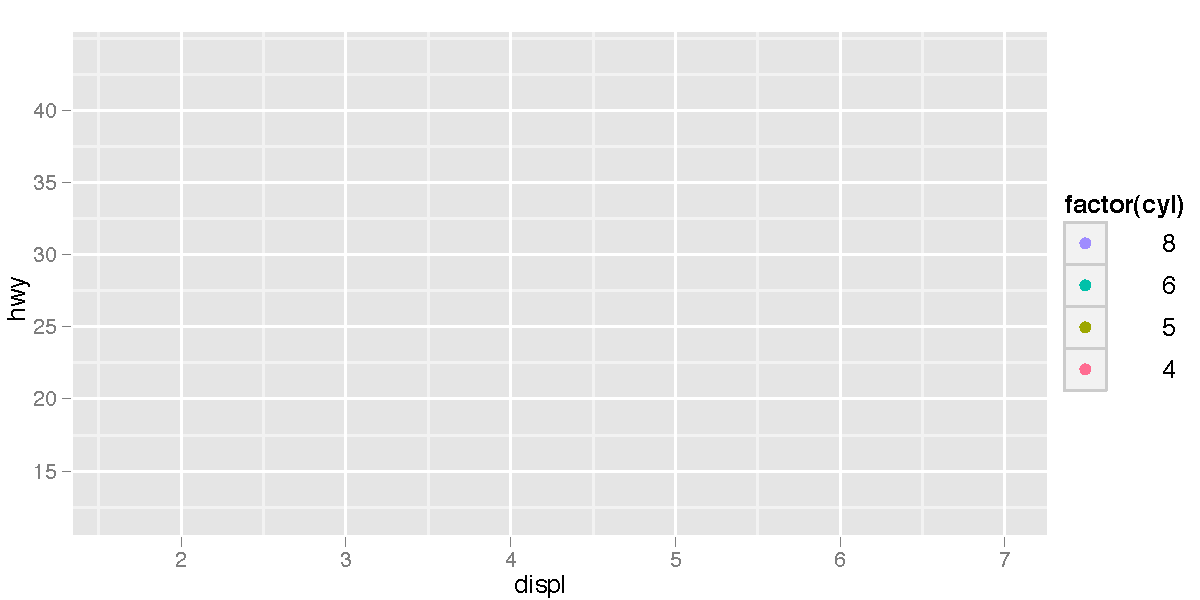
\includegraphics[width=\textwidth]{empty}
  \caption{Contributions from the scales, the axes and legend and grid lines, and the plot background.  Contributions from the data, the point geom, has been removed.}
  \label{fig:empty}
\end{figure}

\section{A more complex plot}
\label{sec:complex-plot} 

With a simple example under our belts, it's now turn to look at the slightly more complicated plot in Figure~\ref{fig:complex}.  This plot adds three new components to the mix: facets, multiple layers and statistics.  The facets and layers expand the data structure described above:  each panel in each layer has its own dataset.  You can think of this as a 3d array: the panels of the facets form a 2d grid, and the layers extend upwards in the 3rd dimension.  In this case the data in the layers is the same, but in general we can plot different datasets on different layers.  Table~\ref{tbl:data-complex} shows the first few rows of the data in each facet.

% scatter2 <- with(mpg, 
%   data.frame(x = displ, y = hwy, colour = cyl, year = year)
% )
% cat(tabulate(subset(scatter2, year == 1999)[1:10, 1:3]))
% cat(tabulate(subset(scatter2, year == 2008)[1:10, 1:3]))

\begin{table}
  \begin{center}
  \begin{tabular}{rrr|rrr}
    \toprule
    \code{x} & \code{y} & \code{colour} & \code{x} & \code{y} & \code{colour} \\
    \midrule
    1.8 & 29 & 4 &  2.0 & 31 & 4\\ 
    1.8 & 29 & 4 &  2.0 & 30 & 4\\
    2.8 & 26 & 6 &  3.1 & 27 & 6\\
    2.8 & 26 & 6 &  2.0 & 28 & 4\\
    1.8 & 26 & 4 &  2.0 & 27 & 4\\
    1.8 & 25 & 4 &  3.1 & 25 & 6\\
    2.8 & 25 & 6 &  3.1 & 25 & 6\\
    2.8 & 25 & 6 &  3.1 & 25 & 6\\
    2.8 & 24 & 6 &  4.2 & 23 & 8\\
    5.7 & 17 & 8 &  5.3 & 20 & 8\\
    \bottomrule
  \end{tabular}
  \end{center}
  \caption{A 1\,$\times$\,2 grid of data frames used for faceting.  In general, this structure also has a third dimension for layers, but in this example the data for each layer is the same.}
  \label{tbl:data-complex}
\end{table}

The smooth layer is different in another respect: it doesn't display the raw data, but a statistical transformation of the data.  This requires an additional step in the process described above: after mapping the data to aesthetics, the data is passed to a statistical transformation, or stat, which manipulates the data in some useful way.  In this example, the stat fits the data to a loess model, and then returns predictions from evenly spaced points within the range of the data.  Other useful stats include 1 and 2d binning, group means, quantile regression and contouring.

% FIGURE
%   GG-WIDTH: 8 GG-HEIGHT: 4 TEX-WIDTH: \textwidth
%   LABEL: complex
%   CAPTION: A more complex plot with facets and multiple layers.
% 
% qplot(displ, hwy, data=mpg, facets = . ~ year) + geom_smooth()
\input{_include/65467dc53c5ef4615b15a004cf82b2e0.tex}
% END

As well as adding an additional step to summarise the data, we also need some extra steps when we get to the scales.  This is because we now have multiple datasets (for the different facets and layers) and we need to make sure that the scales are the same across all of them.  Scaling actually occurs in three parts: transforming, training and mapping.  We haven't mentioned transformation before, but you have probably seen it before in log-log plots.  In a log-log plot, the data values are not linearly mapped to position on the plot, but are first log-transformed.  

\begin{itemize}
  \item Scale transformation occurs before statistical transformation so that statistics are computed on the scale-transformed data.  This ensures that a plot of $\log(x)$ vs $\log(y)$ on linear scales looks the same as $x$ vs $y$ on log scales.  See Section~\ref{sub:coord-transformation} for more details. 
  
  \item After the statistics are computed, each scale is trained on every dataset from all the layers and facets.  The training operation combines the ranges of the individual datasets to get the range of the complete data.  Without this step, scales could only make sense locally and we wouldn't be able to overlay different layers because their positions wouldn't line up.  Sometimes we do want to vary position scales across facets, and this is described more fully in Section~\ref{sub:controlling_scales}.
  
  \item Finally the scales map the data values into aesthetic values.  This is a local operation: the variables in each dataset are mapped to their aesthetic values producing a new dataset that can then be rendered by the geoms.
  
\end{itemize}

Figure~\ref{fig:schematic} illustrates the complete process schematically.

\begin{figure}[htbp]
  \centering
  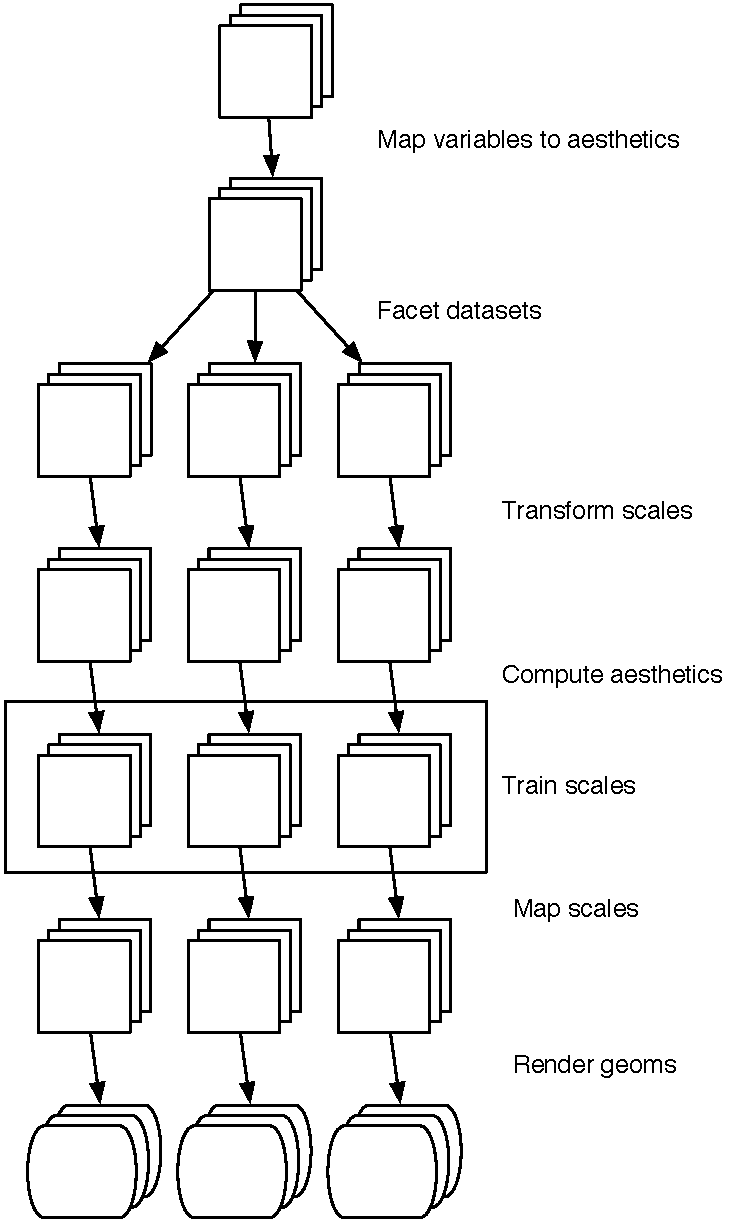
\includegraphics[width=4in]{mastery-schema}
  \caption{Schematic description of the plot generation process.  All steps work by transforming individual data frames, except for training scales which doesn't affect the data frame and operates across all datasets simultaneously.}
  \label{fig:label}
\end{figure}

\section{Components of the layered grammar}
\label{sec:components}

In the examples above, we have seen some of the components that make up a plot:

\begin{itemize}
  \item data and aesthetic mappings,
  \item geometric objects, 
  \item statistical transformations,
  \item scales,
  \item and faceting.
\end{itemize}

\noindent And we have touched on the coordinate system.  Together, the data, mappings, statistical transformation and geometric object form a {\bf layer}.  A plot may have multiple layers, as in the example where we overlaid a  smoothed line on scatterplot.  To pull this all together, the layered grammar defines a plot as the combination of:

\begin{itemize}
  \item A default dataset and set of mappings from variables to aesthetics.
  \item One or more layers, each composed of a geometric object, a statistical transformation, and a position adjustment, and optionally, a dataset and aesthetic mappings.
  \item One scale for each aesthetic mapping.
  \item A coordinate system.
  \item The faceting specification.
\end{itemize}

The layer component is particularly important as it determines the physical representation of the data, with the combination of stat and geom defining many familiar named graphics: the scatterplot, histogram, contour plot, ...  In practice, many plots have (at least) three layers: the data, context for the data, and a statistical summary of the data.  For example, to visualise a  spatial point process, we might display the points themselves, a map giving some context to the locations of points, and contours of a 2d density estimate.  Chapter~\ref{cha:toolbox} describes some of these possibilities in more details.

This grammar is useful for you both as a user and a potential developer of statistical graphics.  As a user, it makes it easier for you to iteratively update a plot, changing a single feature at a time.  The grammar is also useful because it suggests the high level aspects of a plot that \emph{can} be changed, giving you a framework to think about graphics, and hopefully shortening the distance from mind to paper.  It also encourages the use of graphics customised to a particular problem, rather than relying on generic named graphics.

As a developer, the grammar makes it much easier to add new capabilities to \ggplot. You only need to add the one component that you need, and you can continue to use the all of the other existing components.  For example, you can add a new statistical transformation, and continue to use the existing scales and geoms.  It is also useful for discovering new types of graphics, as the grammar effectively defines the parameter space of statistical graphics.

The following sections describe each of the higher level components more precisely, and point you to the parts of the book where they are documented.

\subsection{Layers}

Layers are responsible for creating the objects that we perceive on the plot.  A layer is composed of four parts:  

\begin{itemize}
  \item data and aesthetic mapping,
  \item a statistical transformation (stat), 
  \item a geometric object (geom)
  \item and a position adjustment.
\end{itemize}

\noindent The properties of a layer are described in Chapter~\ref{cha:layers} and how they can be used to visualise data in Chapter~\ref{cha:toolbox}.

\subsection{Scales}\label{sec:scales}

A {\bf scale} controls the mapping from data to aesthetic attributes, and so we need one scale for each aesthetic property used in a layer.  Scales are common across layers to ensure a consistent mapping from data to aesthetics.  Some scales are illustrated in Figure~\ref{fig:scales}.

% FIGURE
%   LABEL: scales
%   CAPTION: Examples of four scales from \ggplot.  From left to right:
%   continuous variable mapped to size and colour, discrete variable mapped to
%   shape and colour.  The ordering of scales seems upside-down, but this
%   matches the labelling of the $y$-axis: small values occur at the bottom.
%   GG-WIDTH: 1  TEX-WIDTH: 1in
% x <- 1:10
% y <- factor(letters[1:5])
% qplot(x, x, size = x) + opts(keep = "legend_box")
% qplot(x, x, 1:10, colour = x) + opts(keep = "legend_box")
% qplot(y, y, 1:10, shape = y) + opts(keep = "legend_box")
% qplot(y, y, 1:10, colour = y) + opts(keep = "legend_box")

A scale is a function, and its inverse, along with a set of parameters.  For example, the colour gradient scale maps a segment of the real line to a path through a colour space.  The parameters of the function define whether the path is linear or curved, which colour space to use (eg. LUV or RGB), and the start and end colours.  

The inverse function is used to draw a guide so that you can read values from the graph.  Guides are either axes (for position scales) or legends (for everything else).  Most mappings have a unique inverse (i.e.\ the mapping function is one-to-one), but many do not.  A unique inverse makes it possible to recover the original data, but this is not always desirable if we want to focus attention on a single aspect.

Chapter~\ref{cha:scales} describes scales in detail.

\subsection{Coordinate system}\label{sec:coordinate_systems}

A coordinate system, {\bf coord} for short, maps the position of objects onto the plane of the plot.  Position is often specified by two coordinates $(x, y)$, but could be any number of coordinates.  The Cartesian coordinate system is the most common coordinate system for two dimensions, while polar coordinates and various map projections are used less frequently.  For higher dimensions, we have parallel coordinates (a projective geometry), mosaic plots (a hierarchical coordinate system) and linear projections onto the plane.

Coordinate systems affect all position variables simultaneously and differ from scales in that they also change the appearance of the geometric objects.  For example, in polar coordinates, bar geoms look like segments of a circle.  Additionally, scaling is performed before statistical transformation, while coordinate transformations occur afterward.  The consequences of this are shown in Section~\ref{sub:coord-transformation}.

Coordinate systems control how the axes and grid lines are drawn.  Figure~\ref{fig:coord} illustrates three different types of coordinate systems.  Very little advice is available for drawing these for non-Cartesian coordinate systems, so a lot of work needs to be done to produce polished output.  Coordinate systems are described in Chapter~\ref{cha:position}.

% FIGURE
%   LABEL: coord
%   CAPTION: Examples of axes and grid lines for three coordinate systems:
%   Cartesian, semi-log and polar. The polar coordinate system illustrates the
%   difficulties associated with non-Cartesian coordinates: it is hard to draw
%   the axes well.
% 
% x1 <- c(1,10)
% y1 <- c(1, 5)
% p <- qplot(x1, y1, geom="blank", xlab=NULL, ylab=NULL) + theme_bw()
% p 
% p + coord_trans(y="log10")
% p + coord_polar()

\subsection{Faceting}\label{sec:intro-faceting}

There is also another thing that turns out to be sufficiently useful that we should include it in our general framework: faceting (also known as conditioning or trellising). This makes it easy to create small multiples of different subsets of an entire dataset. This is a powerful tool when investigating whether patterns hold across all conditions.  The faceting specification describes which variables should be used to split up the data, and how they should be arranged in a grid.  Faceting is described in Chapter~\ref{cha:position}.

\section{Data structures}
\label{sec:data-structures}

These grammar is encoded into R data structures in a fairly straightforward way.  A plot object is a list with components \code{data}, \code{defaults} (the default aesthetic mappings), \code{layers}, \code{scales}, \code{coordinates} and \code{facet}.  The plot object has one another component we haven't discussed yet: \code{options}.  This is used to store the plot specific theme options described in Chapter~\ref{cha:polishing}.  

Plots can be created in two ways: all at once with \f{qplot}, as shown in the previous chapter, or piece-by-piece with \f{ggplot} and layer functions, as described in the next chapter.  Once you have a plot object, there are few things you can do with it:

\begin{itemize}
  \item Render it on screen, with \f{print}.  This happens automatically when
  running interactively, but inside a loop or function, you'll need to
  \f{print} it yourself.
  
  \item Render it to disk, with \f{ggsave}, described in Section~\ref{sec:saving}.

  \item Briefly describe its structure with \f{summary}.
  
  \item Save it a cache copy of it to disk, with \f{save}.  This saves a complete copy of the plot object, so you can easily recreate that exact plot with \f{load}.  Note that data stored inside the plot, so that if you change the data outside of the plot, and then redraw a saved plot, it will not be updated. 
\end{itemize}

\ifwhole
\else
  \nobibliography{/Users/hadley/documents/phd/references}
  \end{document}
\fi